\documentclass[eikonal.tex]{subfiles}

\begin{document}

\begin{figure}
  \centering
  \begin{subfigure}{.5\textwidth}
    \centering
    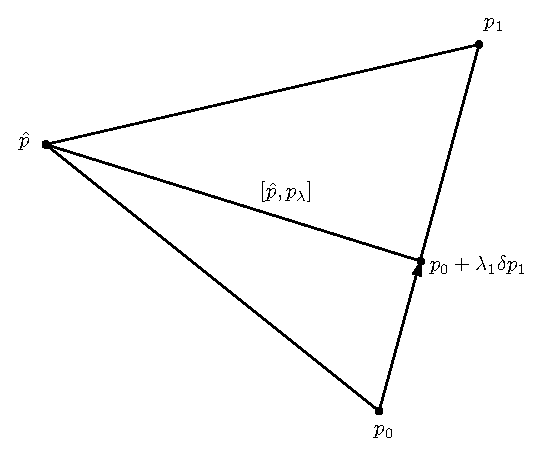
\includegraphics[width=\linewidth]{tri-diagram.eps}
    \caption{An example with $d = 1$ (a triangle
      update).}\label{fig:tri-diagram}
  \end{subfigure}%
  \begin{subfigure}{.5\textwidth}
    \centering
    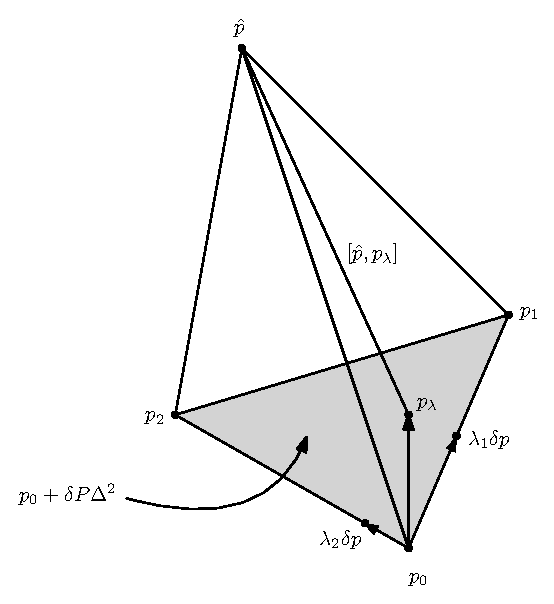
\includegraphics[width=\linewidth]{simplex-diagram.eps}
    \caption{An example with $d = 2$ (a tetrahedron
      update).}\label{fig:tetra-diagram}
  \end{subfigure}
  \caption{Characteristics emanate from the set
    $p_0 + \delta P \Delta^d = \set{p_0 + \lambda_1 \delta p_1 +
      \cdots + \lambda_d \delta p_d}$, which approximates the front of
    the numerical solution.}\label{fig:simplex-diagrams}
\end{figure}

\section{Quadrature Rules}

In this section, we discuss how to compute updates (in
\cref{sec:intro}, \cref{enum:update-U} in our informal description of
the fast marching method). For each update, we identify the updated
point with the origin. We assume our method is operating on a uniform
grid with lattice constant $h$. The vectors $\set{p_0, \hdots, p_d}$
of the previous section are the vectors of the simplex corresponding
to the current update. We assume these vectors are scaled so that, if
$\hat{p}$ denotes the update grid point, then the points which lie on
the (approximate) front of the solution are $\hat{p} + h p_i \in \R^n$
for $i = 0, \hdots, d$. This is useful because on a uniform grid, it
will be convenient for us to work with vectors $p_i$ whose components
satisfy $(p_i)_j \in \set{0, -1, 1}$ for $j = 1, \hdots, n$. In
particular, many of the quantities that we will encounter become
integer-valued and simpler to compute digitally (e.g., the dot product
between two such vectors can be computed rapidly using bitwise
operations).

Each simplex update approximately minimizes a line integral
corresponding to a trial evolution of a characteristic curve of the
numerical solution. We identify the current grid point to be updated
with the origin and denote the trial value of the numerical solution
at this point by $\hat{u}$. In general, we use a hat to denote
quantities for the update point; e.g., below, $\hat{s} =
s(\hat{p})$. We also define $u_\lambda = u_0 + \delta u^\top
\lambda$. Then, the goal is to approximate:
\begin{equation}
  \hat{u} = \min_{\lambda \in \Delta^n} \set{u_\lambda + h \int_{[p_\lambda, 0]} s(\gamma(t))dt}.\label{eq:hat-u-variational}
\end{equation}
using a quadrature rule, where $\gamma$ is an arc length
parametrization of
$[p_\lambda, 0] = \operatorname{conv}(\set{0, p_\lambda})$. We
consider two approximations to \cref{eq:hat-u-variational}: the
difference between the two pertains to the way we incorporate the
slowness function $s$. Let $\theta \in [0, 1]$ and define
$l_\lambda = \norm{p_\lambda}_2$. Then, we define:
\begin{align*}
  F_0(\lambda; \theta) &:= u_\lambda + h s^{\theta} l_\lambda = u_\lambda + h \squareb{(1-\theta)\hat{s} + \frac{\theta}{d + 1} \sum_{i=0}^d s_i} l_\lambda, \\
  F_1(\lambda; \theta) &:= u_\lambda + h s^{\theta}_\lambda l_\lambda = u_\lambda + h \squareb{(1-\theta)\hat{s} + \theta s_\lambda} l_\lambda.
\end{align*}
We will primarily concern ourselves with $F_0$ and $F_1$ for
$\theta = 0$ and $\theta = \nicefrac{1}{2}$. For $\theta = 0$, we have
$F_0 = F_1$, so we define $\Frhr = F_0 = F_1$. On the other hand,
$F_0(\lambda;\nicefrac{1}{2}) \neq F_1(\lambda;\nicefrac{1}{2})$
unless $s \equiv 1$, so we write
$\Fmpzero(\lambda) = F_0(\lambda; \nicefrac{1}{2})$ and
$\Fmpone(\lambda) = F_1(\lambda; \nicefrac{1}{2})$, where ``mp''
stands for ``midpoint''.

\begin{figure}
  \centering
  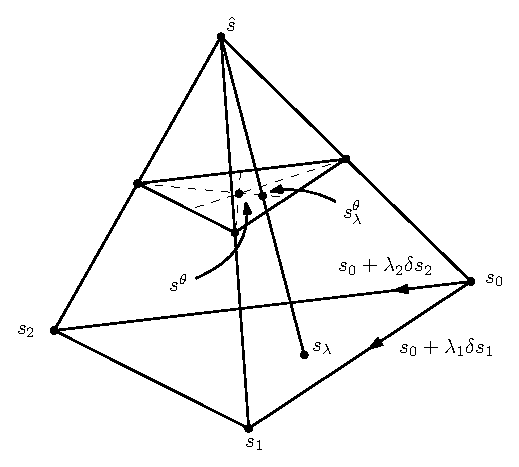
\includegraphics{slowness-tetra.eps}
  \caption{A depiction of the different quantities related to
    $s^{\theta}$ and $s^{\theta}_\lambda$ for the case of $d = 2$, a
    tetrahedron update. Both of $s^\theta$ and $s^\theta_\lambda$ live
    on the $\theta$-section of the simplex
    $\conv \set{\hat{p}, p_0, p_1, p_2}$. The function
    $s^\theta_\lambda$ is a linear combination of $\hat{s}, s_0, s_1$,
    and $s_2$; the value $s^\theta$ is $s^\theta_\lambda$ evaluated at
    the centroid of the $\theta$-section.}
\end{figure}

To compute $\hat{u}$, we will need access to the gradient and Hessian
of $F_0$ and $F_1$. These quantities are easy to compute, but we have
found a particular form for them to be appropriate. We compute these
quantities here.

\begin{lemma}\label{lemma:F0-grad-and-Hess}
  The gradient and Hessian of $F_0(\lambda; \theta)$ satisfy:
  \begin{align}
    \nabla_\lambda F_0(\lambda; \theta) &= \delta u + \frac{s^{\theta} h}{l_\lambda} \delta P^\top p_\lambda, \\
    \nabla^2_\lambda F_0(\lambda; \theta) &= \frac{s^{\theta} h}{l_\lambda} \delta P^\top \calP^\perp_{p_\lambda} \delta P,
  \end{align}
  where $\calP_{p_\lambda}$ denotes the orthogonal projector onto
  $\operatorname{span}(p_\lambda)$ and $\calP_{p_\lambda}^\perp$ is
  the orthogonal projector onto
  $\operatorname{span}(p_\lambda)^\perp$.
\end{lemma}

\begin{proof}
  For the gradient, we have:
  \begin{equation*}
    \nabla_\lambda F_0(\lambda; \theta) = \delta u + \frac{s^{\theta} h}{2 l_\lambda} \nabla_\lambda p_\lambda^\top p_\lambda = \delta u + \frac{s^{\theta} h}{l_\lambda} \delta P^\top p_\lambda,
  \end{equation*}
  since
  $\nabla_\lambda p_\lambda^\top p_\lambda = 2 \delta P^\top
  p_\lambda$. For the Hessian:
  \begin{align*}
    \nabla^2_\lambda F_0(\lambda; \theta) &= \nabla_\lambda \parens{\frac{s^{\theta} h}{l_\lambda} p_\lambda^\top \delta P} = s^{\theta} h \parens{\nabla_\lambda \frac{1}{l_\lambda} p_\lambda^\top \delta P + \frac{1}{l_\lambda} \nabla_\lambda p_\lambda^\top \delta P} \\
    &= \frac{s^{\theta} h}{l_\lambda} \parens{\delta P^\top \delta P - \frac{\delta P^\top p_\lambda p_\lambda^\top \delta P}{p_\lambda^\top p_\lambda}} = \frac{s^{\theta} h}{l_\lambda} \delta P^\top \parens{I - \frac{p_\lambda p_\lambda^\top}{p_\lambda^\top p_\lambda}} \delta P,
  \end{align*}
  from which the result follows.
\end{proof}

\begin{lemma}\label{lemma:F1-grad-and-Hess}
  The gradient and Hessian of $F_1(\lambda; \theta)$ satisfy:
  \begin{align}
    \nabla_\lambda F_1(\lambda; \theta) &= \delta u + \frac{h}{l_\lambda} \parens{\theta p_\lambda \delta s^\top + s^{\theta}_\lambda \delta P}^\top p_\lambda, \\
    \nabla_\lambda^2 F_1(\lambda; \theta) &= \frac{h}{l_\lambda} \parens{\theta \parens{\delta P^\top p_\lambda \delta s^\top + \delta s p_\lambda^\top \delta P} + s^{\theta}_\lambda \delta P^\top \calP^\perp_{p_\lambda} \delta P}. \label{eq:hess-F1}
  \end{align}
\end{lemma}

\begin{proof}
  Since $F_1(\lambda; \theta) = u_\lambda + h s^{\theta}_\lambda l_\lambda$, for the gradient we have:
  \begin{equation*}
    \nabla_\lambda F_1(\lambda; \theta) = \delta u + h \parens{\theta l_\lambda \delta s + \frac{s^{\theta}_\lambda}{2l_\lambda} \nabla_\lambda p_\lambda^\top p_\lambda} = \delta u + \frac{h}{l_\lambda} \parens{\theta p_\lambda^\top p_\lambda \delta s + s^{\theta} \delta P^\top p_\lambda},
  \end{equation*}
  and for the Hessian:
  \begin{equation*}
    \nabla_\lambda^2 F_1(\lambda; \theta) = \frac{h}{2 l_\lambda} \parens{\theta \parens{\nabla_\lambda p_\lambda^\top p_\lambda \delta s^\top + \delta s {(\nabla_\lambda p_\lambda^\top p_\lambda)}^\top} + s^{\theta}_\lambda \parens{\frac{1}{2 p_\lambda^\top p_\lambda} \nabla_\lambda p_\lambda^\top p_\lambda {(\nabla_\lambda p_\lambda^\top p_\lambda)}^\top - \nabla^2_\lambda p_\lambda^\top p_\lambda}}.
  \end{equation*}
  Simplfying this gives us the result.
\end{proof}

% \begin{corollary}
%   \hl{write relationship between $F_1$ gradient and Hessian and $F_0$
%     gradient and Hessian as observation}
% \end{corollary}

% \noindent \hl{\textbf{TODO}: \emph{as an aside, we could use Woodbury
%     or Sherman-Morrison to write $\nabla^2 F_1^{-1}$ in terms of
%     $\nabla^2 F_0^{-1}$. If we came up with a simple way to compute
%     (or precompute and cache) $\nabla^2 F_0^{-1}$, then we might have
%     access to a cheap Newton's method for both $F_0$ and $F_1$. If all
%     we have to do is precompute a QR decomposition for each
%     $\delta P$, and the resulting inverse is correct, the cost of
%     inversion would be $O(nd + d^2) = O(n^2)$ (since $d \leq n$),
%     where $n$ is the dimension of the ambient space and $d$ is the
%     number of vectors $p_i$.}}

\begin{lemma}\label{lemma:dPt-cprojp-dP-pd}
  Let $\Delta^n$ be a nondegenerate simplex. Then,
  $\delta P^\top \mathcal{P}^\perp_{p_\lambda} \delta P$ is positive
  definite.
\end{lemma}

\begin{proof}
  To show that $\delta P^\top \mathcal{P}^\perp_{p_\lambda} \delta P$
  is positive semidefinite, we simply note that since
  $\mathcal{P}^\perp_{p_\lambda}$ is an orthogonal projector, it is
  positive semidefinite, and its singular value decomposition can be
  written $UU^\top$, where $U \in \mathbb{R}^{n+1 \times n}$. Then:
  \begin{equation}\label{eq:dPt-cprojp-dP-gram}
    \delta P^\top \mathcal{P}^\perp_{p_\lambda} \delta P = {(U^\top \delta P)}^\top {(U^\top \delta P)}.
  \end{equation}
  From the factorization in \cref{eq:dPt-cprojp-dP-gram}, we can see
  that $\delta P^\top \mathcal{P}^\perp_{p_\lambda} \delta P$ is a
  Gram matrix, hence positive semidefinite.

  Next, since $\Delta^n$ is nondegenerate, the vectors $p_i$ for
  $i = 0, \hdots, n$ are linearly independent. Since:
  \begin{equation*}
    \delta P = \begin{bmatrix} p_1 - p_0 & \cdots & p_n - p_0 \end{bmatrix},
  \end{equation*}
  the vector $p_0$ is not in the range of $\delta P$; hence, there is
  no vector $\mu$ such that $\delta P \mu = \alpha p_\lambda$, for any
  $\alpha \neq 0$. What's more, by definition,
  $\text{ker}(\mathcal{P}_{p_\lambda}^\perp) = \langle p_\lambda
  \rangle$. So, we can see that
  $\mathcal{P}^\perp_{p_\lambda} \delta P \mu = 0$ only if $\mu = 0$,
  from which we can conclude
  $\delta P^\top \mathcal{P}^\perp_{p_\lambda} \delta P \succ 0$.
\end{proof}

\begin{lemma}
  Again, let $\Delta^n$ be a nondegenerate simplex, and assume that
  $s$ is Lipschitz continuous with constant $K \leq Ch/\sqrt{n}$, for
  some constant $C > 0$. Then, the function $F_0$ is strictly convex
  (i.e., $\nabla^2 F_0$ is positive definite) for all $h > 0$; and, as
  $h \to 0$, the same holds for $F_1$.
\end{lemma}

\begin{proof}
  The fact that $F_0$ is strictly convex follows immediately from
  \cref{lemma:dPt-cprojp-dP-pd} and by noting that
  ${(s^\theta h)}/l_\lambda > 0$. To show that $\nabla^2 F_1$ is
  positive definite for $h$ small enough, note that $\nabla^2 F_1$
  consists of positive definite matrix
  $A = \frac{s^\theta_\lambda h}{l_\lambda}$, plus a small, indefinite
  perturbation,
  $B = \tfrac{\theta h}{l_\lambda} \anticom{\delta P^\top p_\lambda,
    \delta s}$. To use this fact, note that since
  $\delta P^\top \mathcal{P}^\perp_\lambda \delta P$ is symmetric
  positive definite, it has an eigenvalue decomposition
  $Q \Lambda Q^\top$ where $\Lambda_{ii} > 0$ for all $i$. Since
  $\delta P^\top \mathcal{P}^\perp_\lambda \delta P$ doesn't depend on
  $h$, for a fixed set of vectors $p_0, \hdots, p_n$, we can expect
  its eigenvalues to be constant with respect to $h$. So, if we write:
  \begin{equation}
    A = \frac{s^\theta_\lambda h}{l_\lambda} \delta P^\top \mathcal{P}^\perp_\lambda \delta P = Q \parens{\frac{s^\theta_\lambda h}{l_\lambda} \Lambda} Q^\top
  \end{equation}
  we can expect this matrix's eigenvalues to be $\Theta(h)$; in
  particular, $\lambda_{\min} \geq C h$ for some constant $C$,
  provided that $s > \smin > 0$, as assumed. This gives us a bound for
  the positive definite part of $\nabla F_1^2$.

  Now, considering the indefinite perturbation, we can easily see
  that:
  \begin{equation}
    \lambda_{\max}(B) = \norm{\tfrac{\theta h}{l_\lambda} \anticom{\delta P^\top p_\lambda,
        \delta s}} = O(h^2).
  \end{equation}
  Letting $z \neq 0$, we compute:
  \begin{equation}
    z^\top \nabla^2 F_1 z = z^\top A z + z^\top B z \geq \lambda_{\min}(A) z^\top z + z^\top B z \geq Ch z^\top z + z^\top B z.
  \end{equation}
  Now, since
  $\abs{z^\top B z} \leq \abs{\lambda_{\max}(B)} z^\top z \leq D h^2
  z^\top z$, where $D$ is some positive constant, we can see that for
  $h$ small enough, it must be the case that
  $Ch z^\top z + z^\top B z > 0$; i.e., that $\nabla^2 F_1$ is
  positive definite.
\end{proof}

\paragraph{Which simplex should we minimize over?}
\Cref{lemma:F0-grad-and-Hess,lemma:F1-grad-and-Hess} can be formulated
slightly differently. If we take $\Delta^d$ to be the set of $\lambda$
lying in the nonnegative orthant of $\R^{d+1}$ such that
$\sum_{i=0}^d \lambda_i = 1$, then, letting
$P \in \R^{d + 1 \times d + 1}$ so that the $j$th column of $P$ is
$p_i$, we need to define
$F_0(\lambda; \theta) = u^\top \lambda + s^{\theta} h \sqrt{\lambda^\top
  P^\top P \lambda}$. Then:
\begin{equation*}
  \nabla F_0(\lambda; \theta) = u + s^{\theta} h \frac{P^\top p_\lambda}{l_\lambda}, \qquad \text{and} \qquad \nabla^2 F_0(\lambda; \theta) = \frac{s^{\theta} h}{l_\lambda} P^\top \parens{I - \frac{p_\lambda p_\lambda^\top}{p_\lambda^\top p_\lambda}} P.
\end{equation*}
An immediate issue here is that, following this definition,
$\nabla^2 F_0$ becomes singular. Before, the size of $\delta P$
allowed us to mitigate the degeneracy of the orthogonal projection
matrix. This motivates our choice of convention for the convex
coefficients $\lambda$, along with the fact that the smaller dimension
can potentially lead to savings in time and space (however modest).

\end{document}

%%% Local Variables:
%%% mode: latex
%%% TeX-master: "sisc-eikonal.tex"
%%% End:
